%!TEX root = ../presentation.tex

\begin{frame}{Examples}
    \textbf{Example: Triaxial compression test}
\begin{minipage}{1.0\textwidth}
\begin{minipage}{0.55\textwidth}
    \begin{itemize}
        \item Subjected to axial displacement-controlled compression
        \item Different confining pressures (0, 2.5 and 5.0 MPa)
        \item Evolving shear band in the center of the specimen
    \end{itemize}
\end{minipage}
\end{minipage}

\begin{minipage}{1.0\textwidth}
    \begin{figure}[htpb]
        \centering
        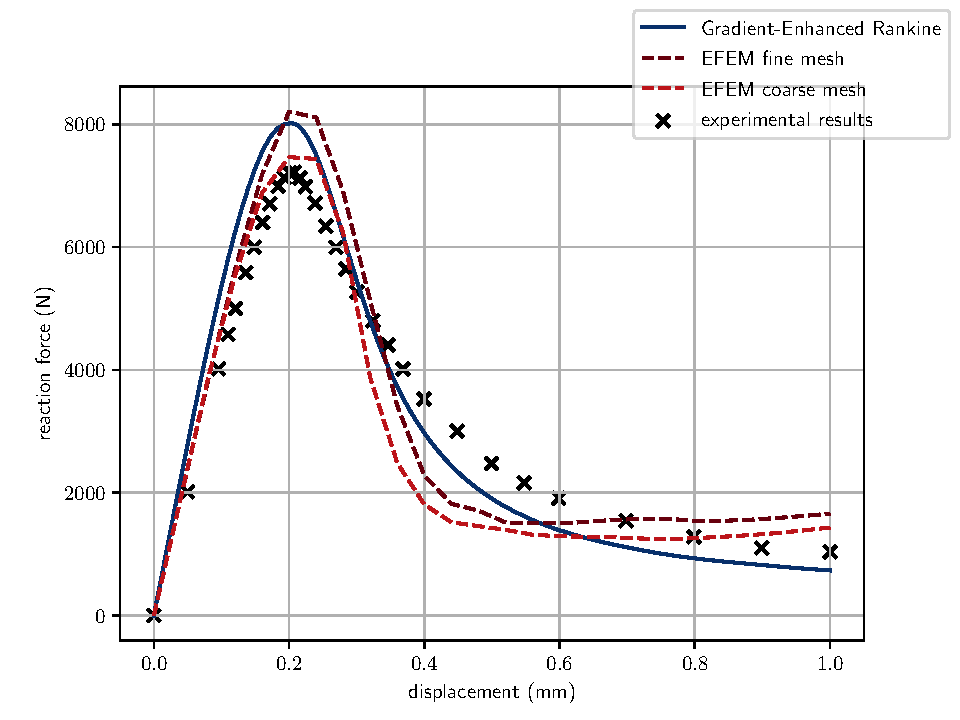
\includegraphics[width=0.6\linewidth]{\slidedir/load_displacement_curves_comparison.pdf}
        \caption{Predicted load-displacement curves by the gradient-enhanced Drucker-Prager model for different confining pressures.}%
    \end{figure}
\end{minipage}
\end{frame}
